The eduROV project aims to let hobbyists, enthusiasts and schools create simple, affordable and open-source underwater ROV's. 

The ROV consisted of a Raspberry Pi 3 Model B+ (RPi) and an Arduino Micro. The Arduino was responsible for reading sensor values and controlling motors. The RPi had multiple tasks, it communicated with the Arduino by reading sensor values and sending motor speed commands. In addition, it captured video from the RPi camera module and displayed this to the user. Lastly, it processed user input from the operator and forwarded these commands to the Arduino.

On the RPi a Python program using the \emph{Pygame}\footnote{\url{https://www.pygame.org/}} package was running. This is an open source package created for making games, but it can also be used to display video feed and read user input. When initiated, this program would display a window on the RPi. \emph{RealVNC}\footnote{\url{https://www.realvnc.com/}}, a software for remote desktop viewing was then used to display this window on the remote computer used for control. \figref{edurovOld} shows this user interface (UI). The software did not require any installation, instead the correct files had to be copied from a GitHub repository.

\begin{figure}[h!]
    \centering
    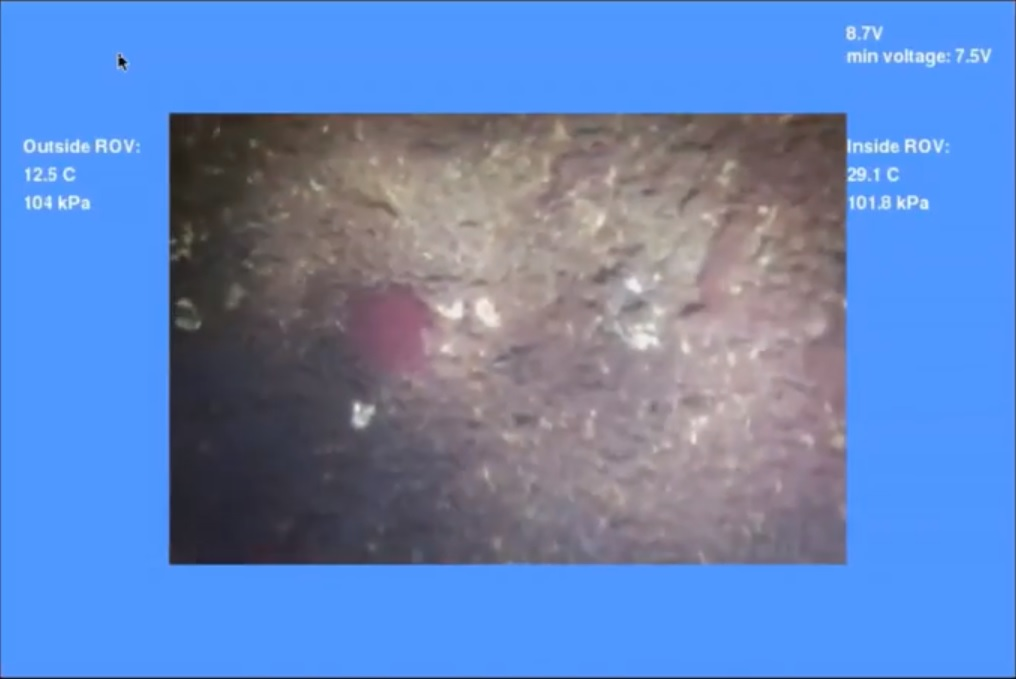
\includegraphics[width=0.8\textwidth]{edurovOld}
    \caption{User interface for the original eduROV software.}
    \label{edurovOld}
\end{figure}

Five main goals were set for my contribution to the project:

\begin{itemize}
\item Reduce the video latency as much as possible while still having the possibility for high resolution images.

\item Streamline the installation process, i.e. remove the need for visiting any website or manually coping files.

\item Remove the need for any third party applications, that would mean removing the RealVNC dependency for video transfer.

\item Increase customization while still maintaining a high level application programming interface (API).

\item Make the UI more attractive, include more UI features without overwhelming the operator.
\end{itemize}

\section{Current alternatives}

There exists a wealth of software's created for operating ROV's. This discussion will be limited to those that are open source and created in Python. The most well known and probably most used is the \emph{Robot Operating System} (ROS)\footnote{\url{http://www.ros.org/}} which is ported to Python as a client library called \emph{rospy}\footnote{\url{http://wiki.ros.org/rospy}}. Although a powerful framework, it does not not suit the needs of this project. Originally written C++, ROS was originally not created for Python. This means that the documentation is mostly in C++ and for anyone who wanted to customize the eduROV software in the future would have learn ROS in addition to Python. It was decided that making ROS fit the needs of the eduROV project would require more time and be limiting to the development, in comparison to creating a tailored software from scratch.

There is also a software called \emph{GoPiGo}\footnote{\url{https://www.dexterindustries.com/gopigo3/}}. This started as a Kickstarter project and is now a hardware and software project that you can buy online. It provides robot communication with video feed, but the software seems to be created specifically for the robots they sell and not as a package meant for other users to build on.

In summary, there wasn't really any good software alternatives for the eduROV project. Actually, I was not able to find any Python packages created for ROV communication with video support built in. There are many guides on the internet that will walk you through how to create this, but the whole process can be really intimidating for people with limited experience. In addition, many of the guides online require you to install multiple software's and download files from additional places. Not very user friendly. Also, in the guides online they often control ROV's by pushing buttons on a screen, not by keyboard input. Lastly, they contain limited to none documentation.

\section{Development}

All popular and well known packages in the Python community is developed in correspondence with the \emph{Python Packaging User Guide}\footnote{\url{https://packaging.python.org/}}. This guide establishes multiple rules on how packages should be developed and distributed. In comparison it is always possible to upload code to a remote repository and ask people to download it from there. But there are many good reasons why any serious actors use this method. 

By distributing code through the \emph{Python Package Index}, anyone can install the package by running \texttt{"pip install edurov"} in a terminal. No need to visit any websites or copy any files. This command will download and install the required files automatically. Second reason is that this greatly simplifies the process of documentation. By creating special files as stated by the guidelines, a separate website with all the documentation is created and uploaded automatically. It also specifies rules for a versioning scheme. This let's the developer create alpha, beta, release candidates and deployment versions of the software. It makes it easy to make sure that everything is tested properly before it get's publicly available.

Git version control was used throughout the project. All the code was uploaded to the remote repository at \url{https://github.com/trolllabs/eduROV}. Git branches was used for rapid prototyping of different ideas. This meant that different approaches were developed concurrently in each their branch. They were then removed one after another as it became clear that the approach did not meet the requirements. The finished package code can also be seen in the appendix.

In the first phase of the development two main methods were tested. The first method was based upon the \emph{pygame} package. It required the operator to install Python and the eduROV package on both the ROV and the controlling computer itself. When the software was started a program window would pop up on the controlling computer and display the video feed. Any customization to the features and UI would require the user to learn pygame since all the graphics are created using the pygame API. The original software also used pygame, but this approach did not rely on RealVNC for transmission. Instead it used socket communication to transfer data.

The second method was based upon a web server approach. This method served a web page from the ROV which could then be viewed on any device connected to the same network as the ROV. This meant that the operator would not have to install any software on his or hers computer. It also meant that the UI would be created using html and css instead of pure pygame. This approach were chosen for the new eduROV package. It would completely remove the need to install anything on the operators computer. It would make it possible to view the video stream at multiple devices at the same time. In addition, web browsers has been around for a very long time and much effort has been spent on making them as efficient and flexible as possible. By using the browser as a medium it's possible to take advantage of this. Some high schools also have web development and html as part of their curriculum. By basing the the eduROV package on a web server framework it becomes possible to let the operator customize the UI with their knowledge of html and css.

When the main method were chosen, proceeding development were administered through the \emph{GitHub issues workflow}\footnote{\url{https://github.com/trolllabs/eduROV/issues}}. \figref{issues} shows a section of the \emph{issues} page on GitHub. On this page, feature requests and bug descriptions were posted by me and one other that tested the software. These were then completed in turn and uploaded as \textit{commits} and \textit{releases}.

\begin{figure}[h!]
    \centering
    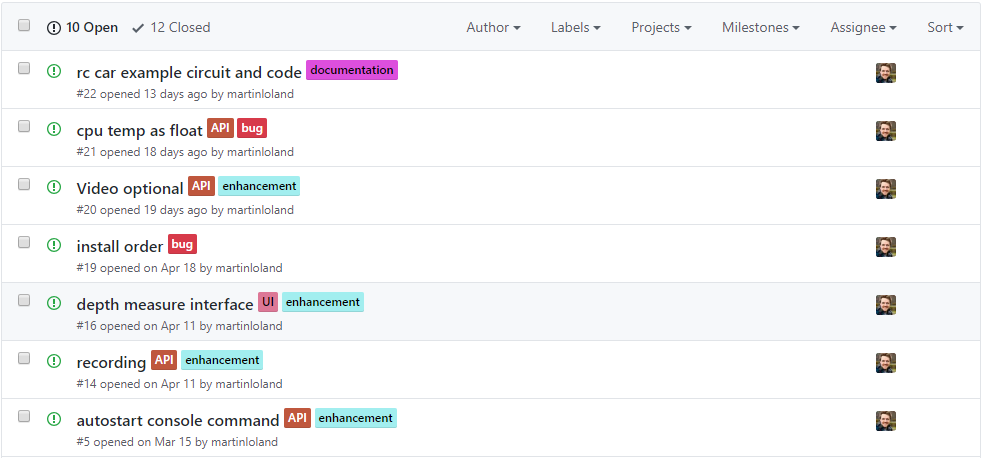
\includegraphics[width=0.8\textwidth]{issues}
    \caption{GitHub eduROV issues overview.}
    \label{issues}
\end{figure}

\section{Architecture}

The eduROV package is based upon a HTTP web server framework. This means that any information sent between the ROV and the user is communicated though HTTP GET requests. For increased performance and robustness many of the different tasks are spread on multiple processes running in parallel. This ensures utilization of multiple CPU cores. The Pyro4\footnote{\url{https://pythonhosted.org/Pyro4/}} Python package uses socket TCP communication and were chosen to facilitate transfer of data between processes. It's fast, well maintained and easy to use.

\figref{edurovArchitecture} pictures the flow of information between different processes and parts of the system. When the user interact with the keyboard, this is sent as a HTTP request from the web browser to the web server on the ROV. This is a threaded HTTP server, which means that multiple requests can be handled at the same time in different computer threads. The web server will forward this information to the \textit{synchronize process} which is responsible for holding an updated version of all variables. The \textit{Arduino process} checks the synchronize process many times per second and forwards any new key presses to the Arduino through a serial connection, which then moves the motors correspondingly. Sensor values moves in a similar fashion, only in the opposite direction. The camera captures frames, compresses them to .jpg files and store them in a memory buffer. The webserver will then send the image to the web browser as soon it is ready, directly from the buffer. Lastly, the \textit{system monitor process} regularly checks that the drive space and CPU temperature is ok and notifies the synchronize process.


\begin{figure}[h!]
    \centering
    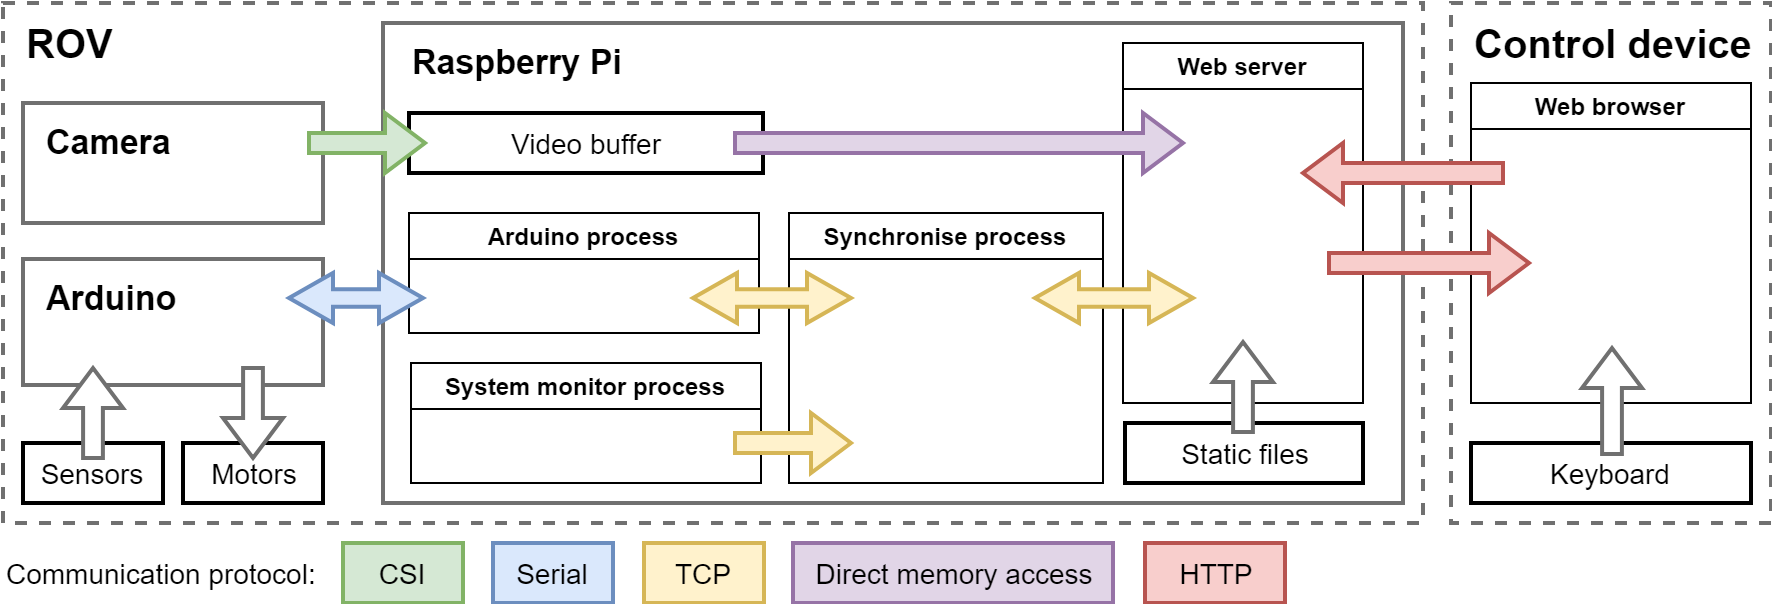
\includegraphics[width=\textwidth]{edurovArchitecture}
    \caption{System architecture of the eduROV software.}
    \label{edurovArchitecture}
\end{figure}

\section{Graphical user interface}

\figref{edurov_gui} shows the finished UI. The layout is dynamic which means that it will fit any screen size and ratio. The side panels will stay the same size but the video will shrink and increase in size to what's available. Left panels shows sensor values from the Arduino and RPi. Center section shows the video feed. There is also a roll indicator that shows how the ROV is oriented in the water. This indicator can be toggled on/off from the button menu in the right panel. From this panel the operator has multiple options, such as to arm the robot. If the robot is not armed it will not move. Cinema mode will hide all panels and scale the video feed to it's maximum size. Some of the actions can also be triggered with hotkeys. With this layout, the user can chose whether to view all information or nothing except the video feed. An approach with information in side panels was chosen because \citet{Chen2007} argued that "overlaying information on video feed can potentially lead to cognitive tunnelling".

\begin{figure}[h!]
    \centering
    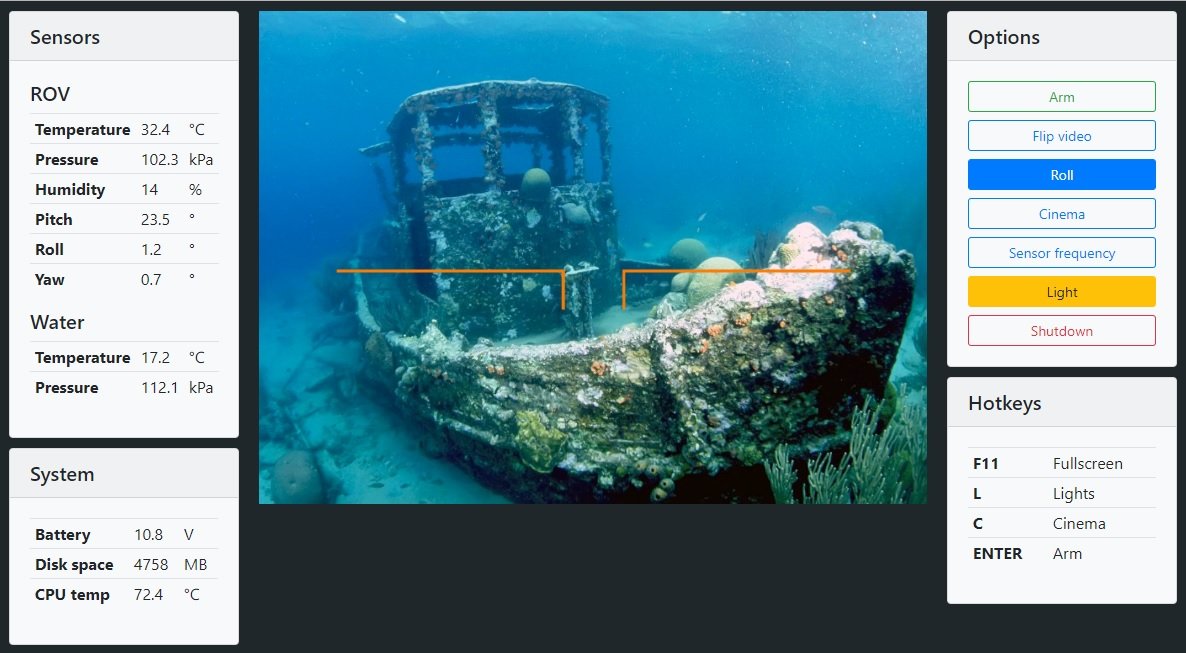
\includegraphics[width=0.8\textwidth]{edurov_gui}
    \caption{The graphical user interface in the eduROV package.}
    \label{edurov_gui}
\end{figure}

The UI seen above is in the context of the Engage eduROV submersible. But since the UI is created purely in HTML, CSS and JavaScript, any user of the package can customize the look and feel of the webpage in any way he or she would like. In fact, a completely different UI was created for the experiment in chapter \ref{chpMethod}, but still used the eduROV framework for handling requests.

\section{Application programming interface}

The application programming interface (API) is how the user interact with the software package. One of the goals of the project was to create an API that would get the user up an running in a matter of minutes. In addition, provide a flexible API that provides extensive flexibility and customization. There is one single main class called \texttt{WebMethod}. By initiating this class with the path to the \texttt{index.html} file which decribes the layout, the web server will start running and serving the web page and video feed. In addition to that, the user is able to customize which functions that should be started in their own processes, custom responses to GET methods, resolution and frame rate and much more.

The reader is recommended to take a look at the API\footnote{\url{http://edurov.readthedocs.io/en/latest/api.html}} and getting started\footnote{\url{http://edurov.readthedocs.io/en/latest/started.html}} section of the documentation. These pages describes the API and provide a much better user experience than what can be provided in a book. 


\section{Documentation}


The documentation is written using the \emph{reStructuredText}\footnote{\url{http://docutils.sourceforge.net/rst.html}} markup syntax and compiled using the Sphinx\footnote{\url{http://www.sphinx-doc.org/}}. This enables in-line program documentation. This is very helpful because the documentation for the classes, methods and functions can be written in the same place as the actual code. This creates fewer files which are easier to maintain. In addition, sphinx will automatically detect classes, functions and methods and create a corresponding documentation structure.

The GitHub repository has been connected to an account at \emph{readthedocs.io}. By connecting these accounts, a documentation website is automatically created from the sphinx structure when updates are committed to the repository. The documentation can be seen online\footnote{\url{http://edurov.readthedocs.io}} or in the appendix. A sample can be seen in \figref{docs}.

\begin{figure}[h!]
    \centering
    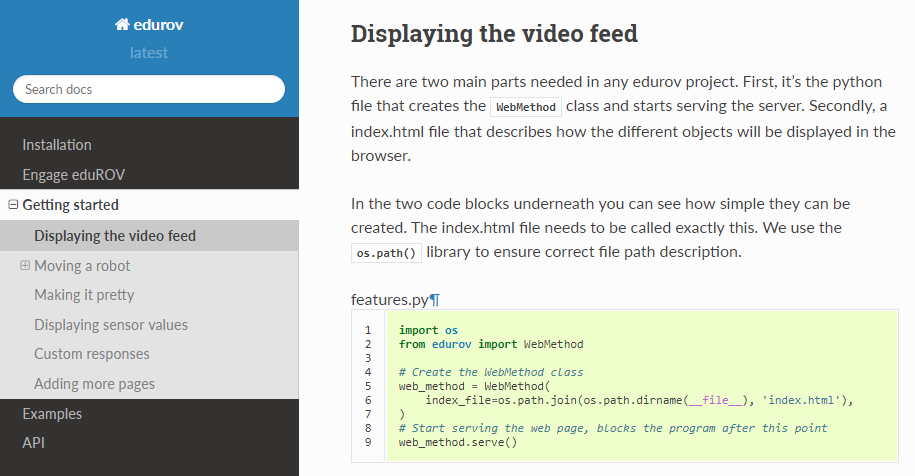
\includegraphics[width=0.8\textwidth]{docs}
    \caption{eduROV documentation at readthedocs.io}
    \label{docs}
\end{figure}
\clearpage
\section{Performance and novelty features}

\begin{figure}[h!]
    \centering
    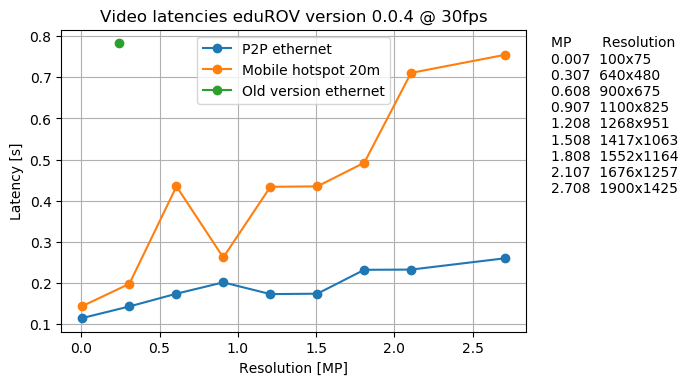
\includegraphics[scale=0.7,right]{latency}
    \caption{Video latency for eduROV 0.0.5 \@ 30fps.}
    \label{latency}
\end{figure}

\figref{latency} shows a delay performance test that were performed on version 0.0.5 of the eduROV package. With a resolution of 0.3 mega pixels on a wired ethernet connection, the video latency has been reduced from 782ms to 143ms. This is a 82\% reduction. It is even possible to stream full HD video with a latency below 300ms. When using wireless transmission the latency is affected by factors such as distance, interference and hardware. The test was performed in the same way as \citet{Jennhag2016} did in their test. By manually comparing two timers, one in real time on the monitor and the other as captured by the camera and transmitted back to the same monitor.

A summary of the most novelty features in comparison with other similar solutions can be listed as follows:

\begin{itemize}
\item Low video latency. Possibility to stream high definition video with a delay below 200ms.

\item No setup required. The controlling computer does not need any software installed. The ROV can even be controlled from a mobile phone.

\item Very easy to use. One command in the terminal window will install all required files. One additional command will start the web server.

\item Highly customizable. Since the UI is created in html the user can customize the look and feel of the web page in any way.

\item Easy true parallelism. Custom functions can be spawned on multiple CPU cores while still maintaining the possibility to share variables.

\end{itemize}

For future work there is one limitation to the current design. The client browser communicates with the web server with GET requests. Each time the UI is updated, the client has to ask for this update, there is no way that the server can send new information to the client on it's own. This is unless a \emph{WebSocket} connection is used. Instead of creating a new connection each time a request is done, a websocket is open as long as the client is viewing the web page. This enables the server to push information when it have something new and thus removing a lot of unnecessary communication. This would require some big changes to the underlying workings of the eduROV package, but is probably where the next big performance gain can be achieved.